\chapter{Methodology and Practical Analysis of the Fusee Gelee Exploit}
\epigraph{quote}{\textit{author}}

\section{Research Approach}

In this chapter we'll start with the Methodology on how to get past the securities of the Nintendo Switch, and the Fusee Gelee exploit. This will helps gather insights into current knowledge, identify gaps, and understand the significance of the Fusee Gelee exploit.

\subsection{Technical Analysis}

The technical analysis involves a detailed examination of the Fusee Gelee exploit. This includes studying the specifics of the vulnerability, understanding the exploitation process, and analyzing the implications. Documentation and code analysis are critical for a deep understanding of the exploit and its impact on the Nintendo Switch's security.

\subsection{Experimentation}

Practical experimentation is conducted to replicate and analyze the Fusee Gelee exploit using the methods detailed on the Switch Guide. This involves setting up a controlled environment to safely execute the exploit on a Nintendo Switch device, validating theoretical findings, observing the exploit, and gathering empirical data on its effects.

\section{Experimental Setup and Execution}

\subsection{Tools and Materials}

The experimental setup requires specific tools and materials, including:

\begin{itemize}
    \item A Nintendo Switch device vulnerable to the Fusee Gelee exploit.
    \item A computer with USB connectivity to interface with the Switch.
    \item Software tools for sending the malicious USB payloads, such as TegraRcmGUI.
    \item An RCM jig to force the Switch into recovery mode.
\end{itemize}

\subsection{Procedures}

The procedures for executing the Fusee Gelee exploit are detailed as follows:

\begin{itemize}

    \item \textbf{Preparing the Device}: The Switch is prepared by entering Recovery Mode (RCM). This is achieved using an RCM jig, a simple tool that connects specific pins on the Joy-Con connector. The 3D model for the RCM jig can be found on Makerworld\cite{NintendoSwitchJig}.

   % inline 2 images side by side
   \begin{figure}[H]
       \centering
       \begin{minipage}{.5\textwidth}
           \centering
           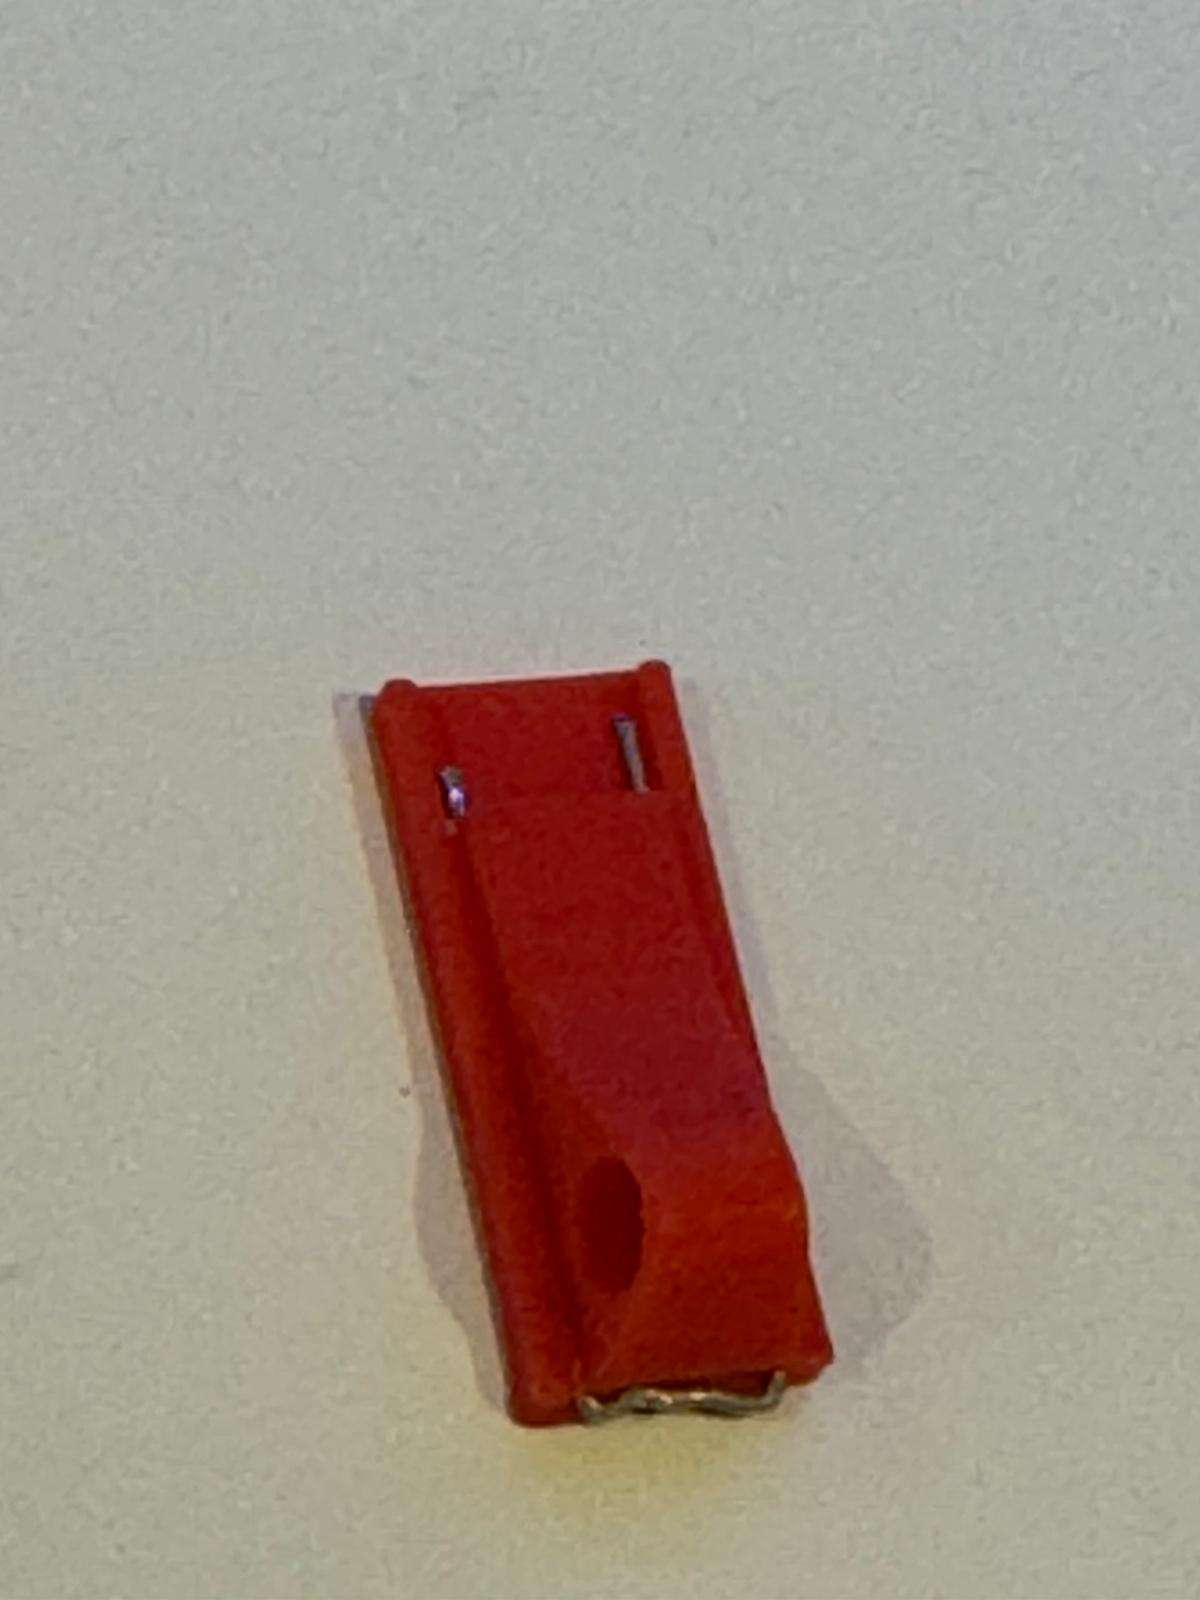
\includegraphics[width=.8\linewidth]{images/rcm_jig.jpg}
           \captionof{figure}{RCM Jig}
           \label{fig:rcm_jig}
       \end{minipage}%
       \begin{minipage}{.5\textwidth}
           \centering
           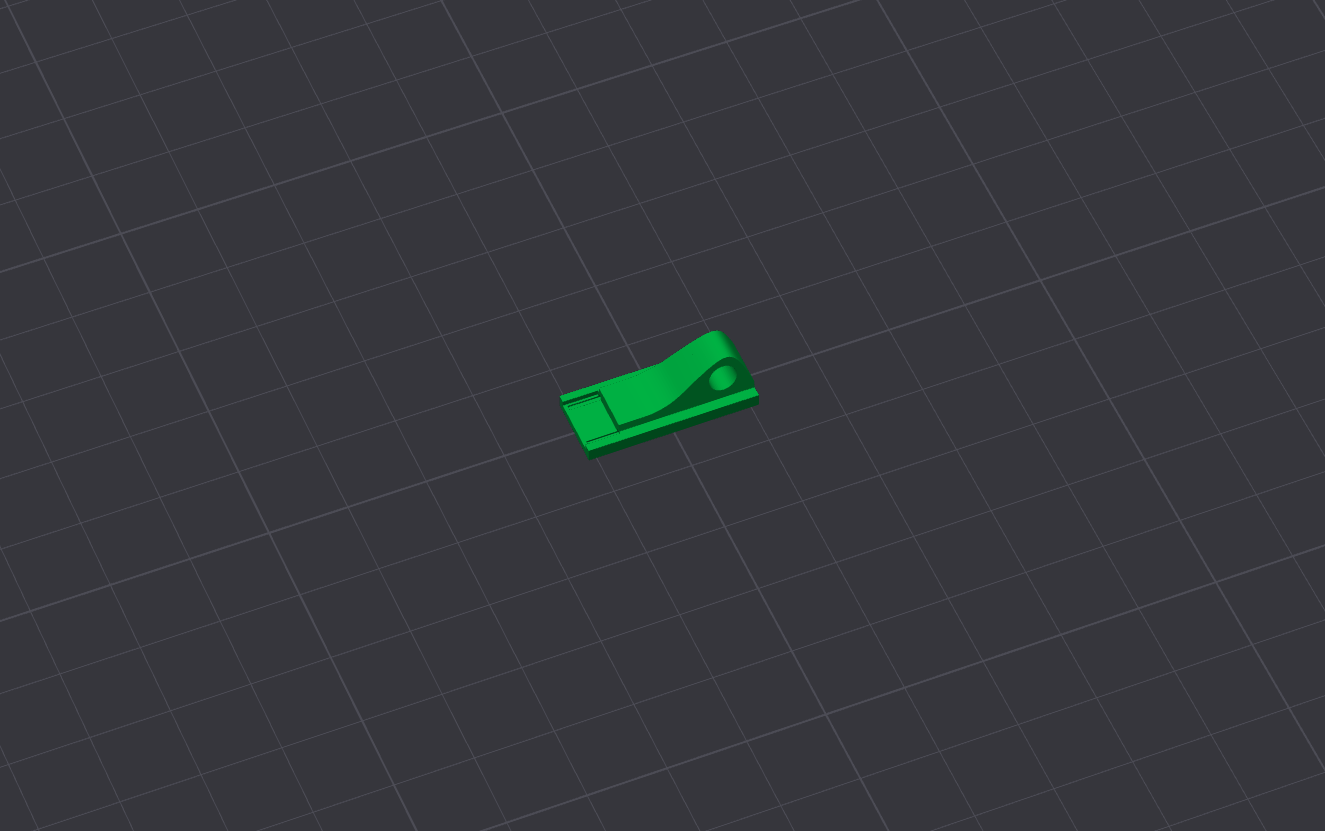
\includegraphics[width=.8\linewidth]{images/nintendo_jig.png}
           \captionof{figure}{RCM Jig 3D Model}
           \label{fig:switch_rcm}
       \end{minipage}
    \end{figure}

    \item \textbf{Connecting to the Computer}: The Switch is connected to the computer via USB. TegraRcmGUI is used to send the exploit payloads.

   % inline 3 images no rcm, yes rcm payload sent
    \begin{figure}[H]
         \centering
         \begin{minipage}{.4\textwidth}
              \centering
              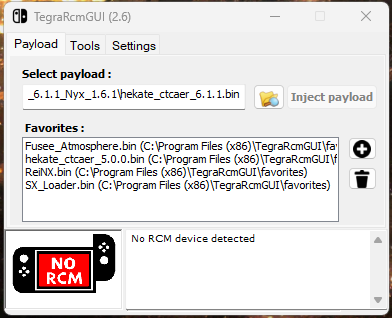
\includegraphics[width=.8\linewidth]{images/no_rcm.png}
              \captionof{figure}{No RCM Detected}
              \label{fig:no_rcm}
         \end{minipage}%
         \begin{minipage}{.4\textwidth}
              \centering
              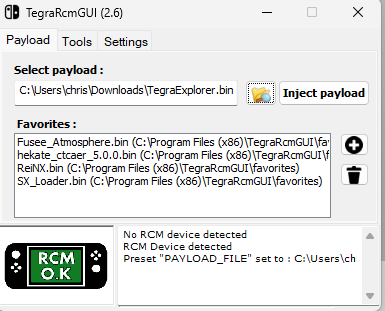
\includegraphics[width=.8\linewidth]{images/yes_rcm.png}
              \captionof{figure}{RCM Detected}
              \label{fig:rcm_detected}
         \end{minipage}%
    \end{figure}
    \begin{figure}[H]
        \centering
        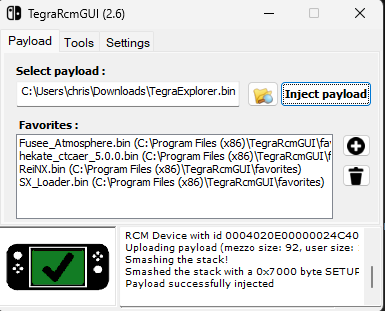
\includegraphics[width=.3\linewidth]{images/payload_sent.png}
        \caption{Payload Sent}
        \label{fig:payload_sent}
   \end{figure}

    \item \textbf{Sending the Payloads}: Two payloads are required. The first payload (Tegra Explorer) is used to partition the SD card so we can create the necessary partitions to run the emulated system without losing the stock one. The second payload, Hekate, contains the bootloader and the custom firmware.
\end{itemize}

\section{Analysis}

\subsection{Results Interpretation}

The results from the practical experimentation provide valuable insights into the effectiveness and impact of the Fusee Gelee exploit. One of the key findings is the validation of the exploit's capability to bypass the secure boot process. This validation is crucial as it demonstrates that the exploit can successfully subvert the intended security mechanisms of the Nintendo Switch, allowing for arbitrary code execution. By confirming this aspect, the experiment highlights the fundamental vulnerability within the Tegra X1 chip's Boot ROM.

\begin{figure}[H]
    \centering
    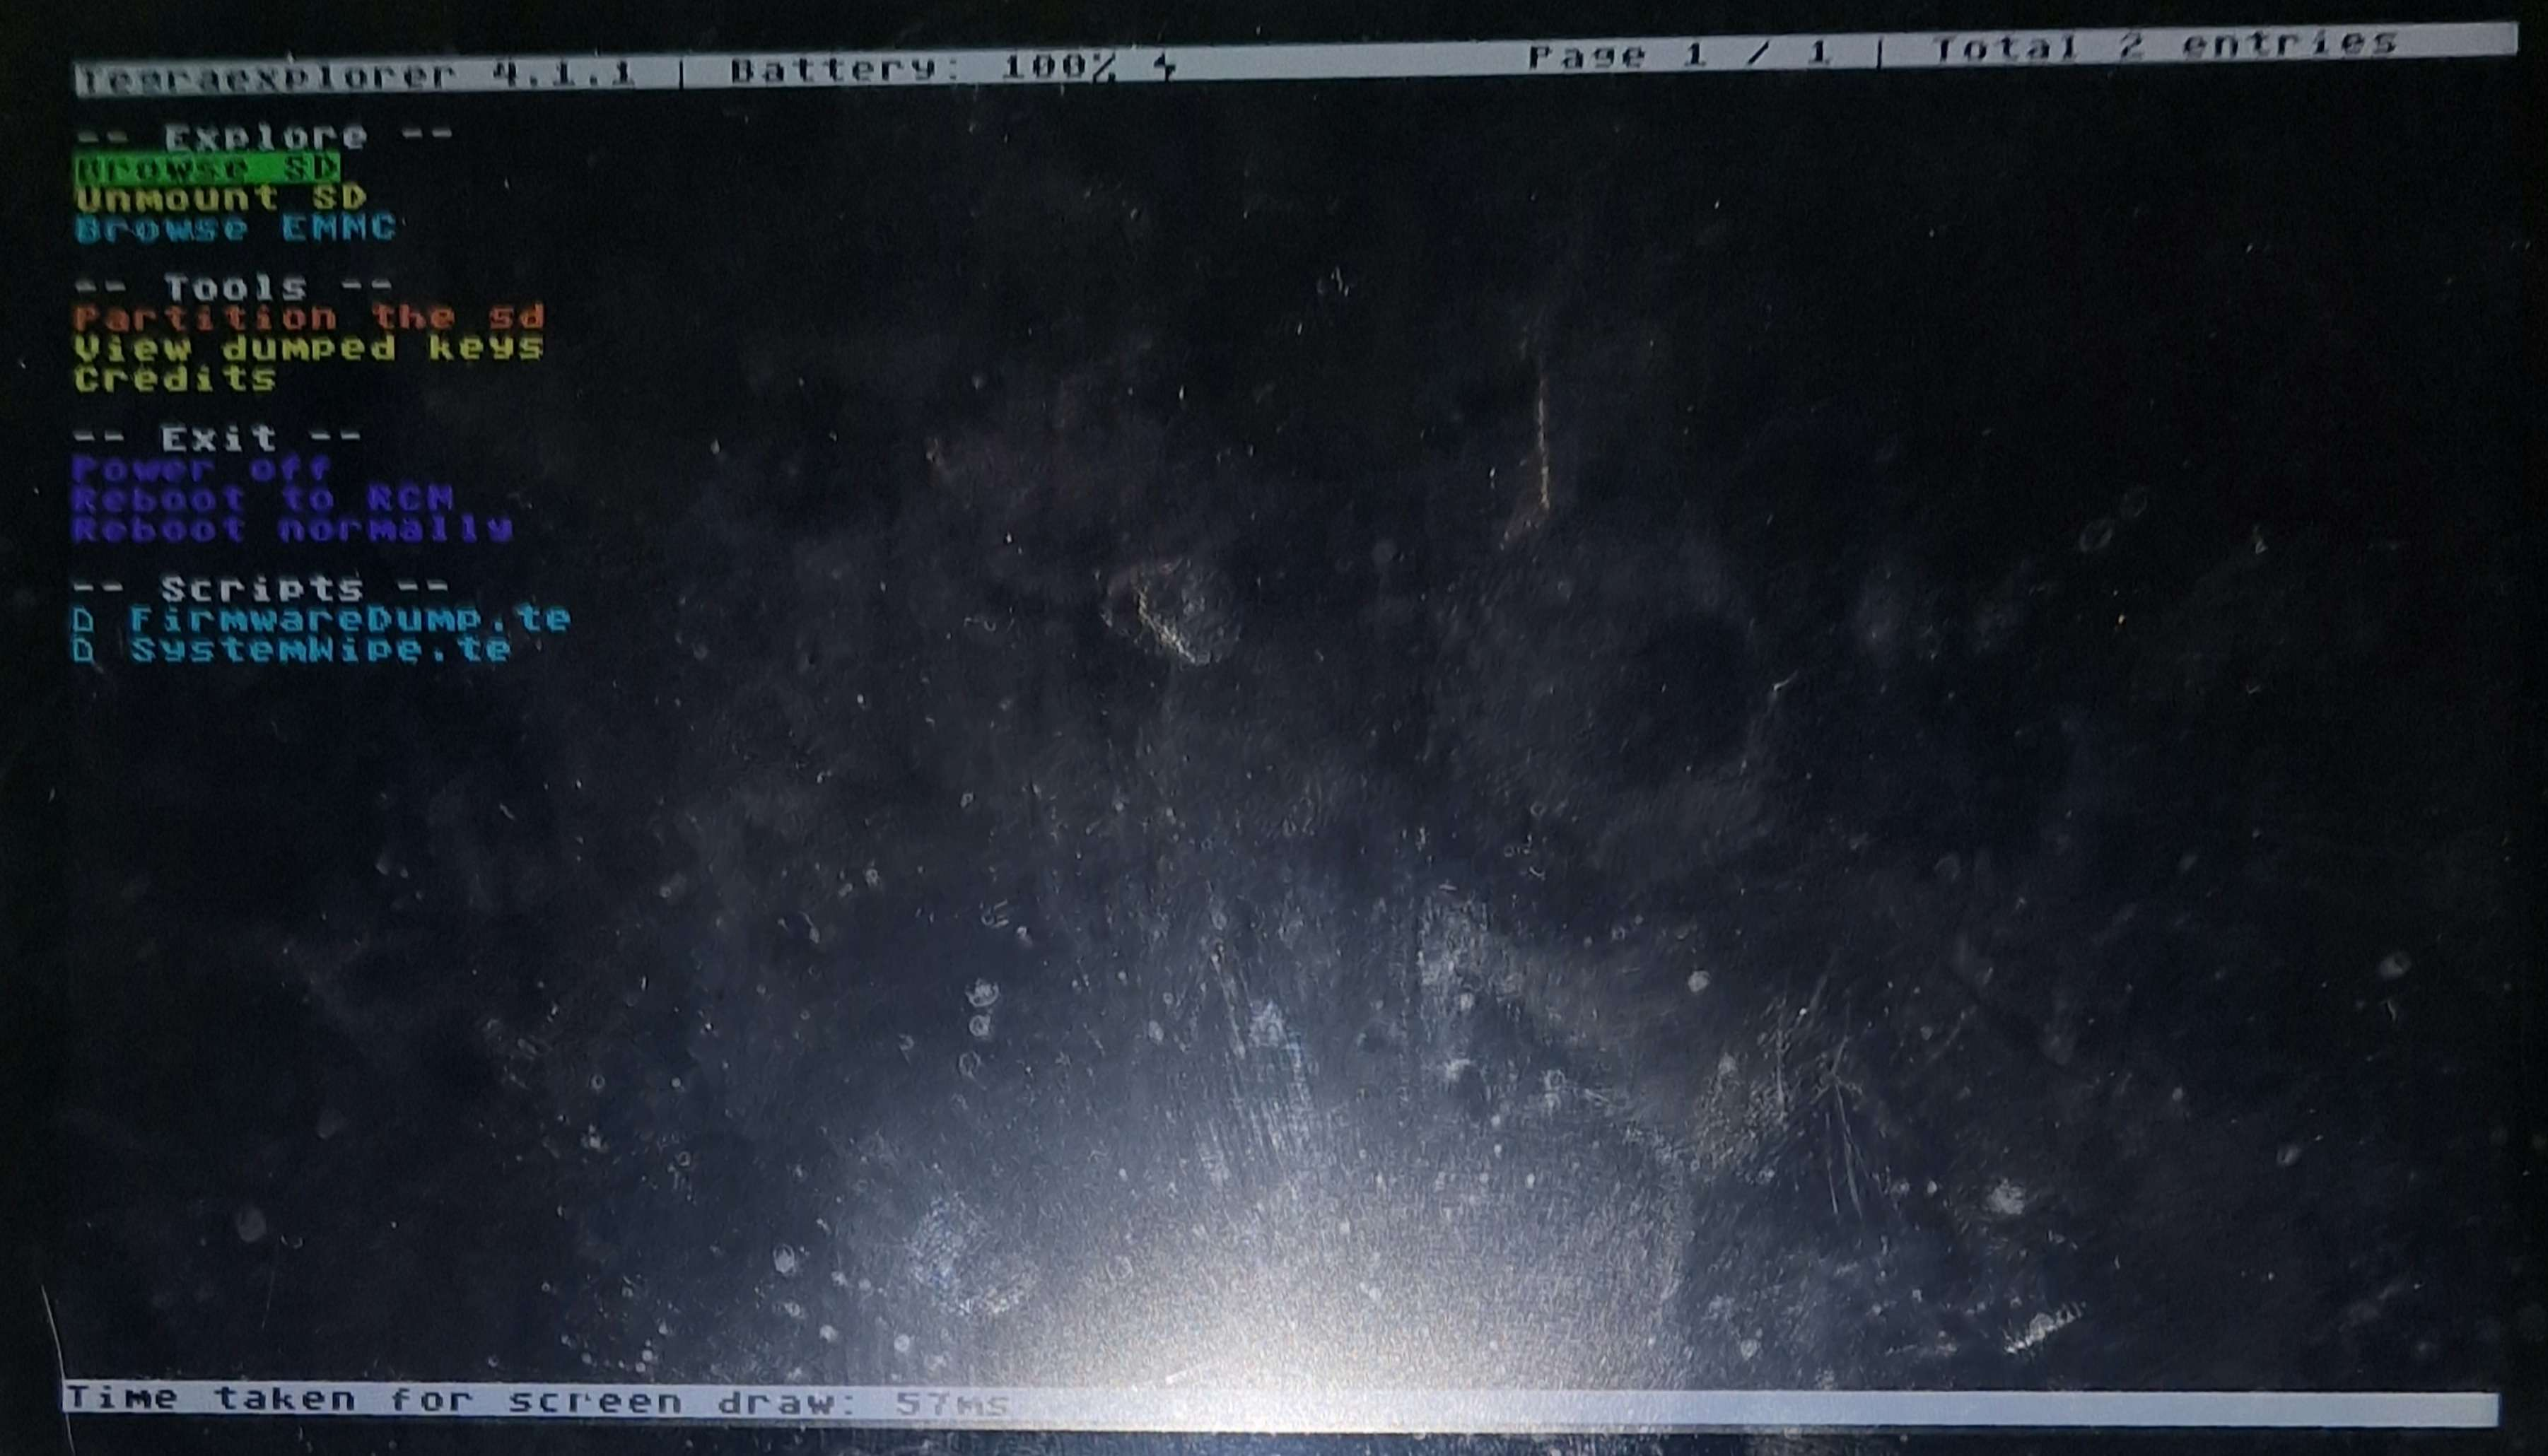
\includegraphics[width=.8\linewidth]{images/tegra_explorer.jpg}
    \caption{Nintendo Switch Running Tegra Explorer}
    \label{fig:switch_boot}
\end{figure}

\subsection{Discussion of Significance}

The significance of the findings from the Fusee Gelee exploit extends beyond the immediate technical details, impacting broader hardware security concerns (like other devices using the same chip). One major implication for device security is the clear demonstration of how a single vulnerability in a critical component like the Boot ROM can undermine the entire security architecture of a device. This highlights the need for rigorous security measures and thorough testing during the hardware design phase to prevent such vulnerabilities from being embedded in the final product.

From this analysis, several lessons can be drawn for hardware manufacturers. Firstly, the importance of thorough security testing is paramount. Manufacturers must ensure that every component, especially those involved in the secure boot process, is rigorously tested for vulnerabilities. This involves not only initial testing but also ongoing assessments as new threats emerge. Secondly, the findings underscore the need for robust mitigation strategies. Once a vulnerability is discovered, manufacturers must be prepared to implement comprehensive measures to address it, which may include hardware revisions, software updates, and in some cases, recall or replacement of affected devices.

In conclusion, the Fusee Gelee exploit serves as a critical case study in the field of hardware security. It exemplifies the challenges associated with detecting and mitigating hardware vulnerabilities and underscores the importance of proactive security measures. The insights gained from this analysis provide valuable guidance for improving the security of future hardware designs, ensuring that devices are resilient against similar threats.